\chapter{Analysis}\label{chap:analysis}
\section{Forward proton selection}
\section{Event and track selection}
\subsection{Event selection}
\subsection{Track selection}
\section{Accidental background study}

The accidental backgrounds (same bunch pile-up background) are quantified using data-driven method. This includes any single(double)-side proton signal collected in coincidence with a diffractive like signal in the TPC-TOF detector. This type of background may come from the overlap of:
\begin{enumerate}
	\item RP:
	\begin{itemize}
		\item proton from beamhalo,
		\item low mass SD process without activity in TOF,
		\item elastic or low mass CD processes with undetected proton on the other side,
	\end{itemize}
	\item TPC+TOF:
	\begin{itemize}
		\item any central activity (dominantly from ND events).
	\end{itemize}
\end{enumerate}
\subsection{Proton overlay probability}
The probability of observing the protons passing the RP proton track selection of the analysis  was calculated from \textbf{Zerobias} trigger sample. As being assumed to be uncorrelated to the TPC-TOF activity, the probability is used to quantify the addition of an extra-proton to any kind of events. Figure \ref{fig:probSD} shows the derived probabilities of getting global and local proton tracks in SD. The probabilities of observing two protons on the opposite sides of the IP in CD using only proton global tracks were shown in the Figure \ref{fig:probCD}.  The main contribution to the accidental background in CD comes from the inelastic RP configuration, where it is dominated by elastic (halo), elastic and SD, halo and SD protons and its probability equals to about $0.2\%$.
\begin{figure}[H]
	\centering
	\parbox{0.48\textwidth}{
		\centering
		\begin{subfigure}[b]{\linewidth}{
				\subcaptionbox{\label{fig:probSD}}{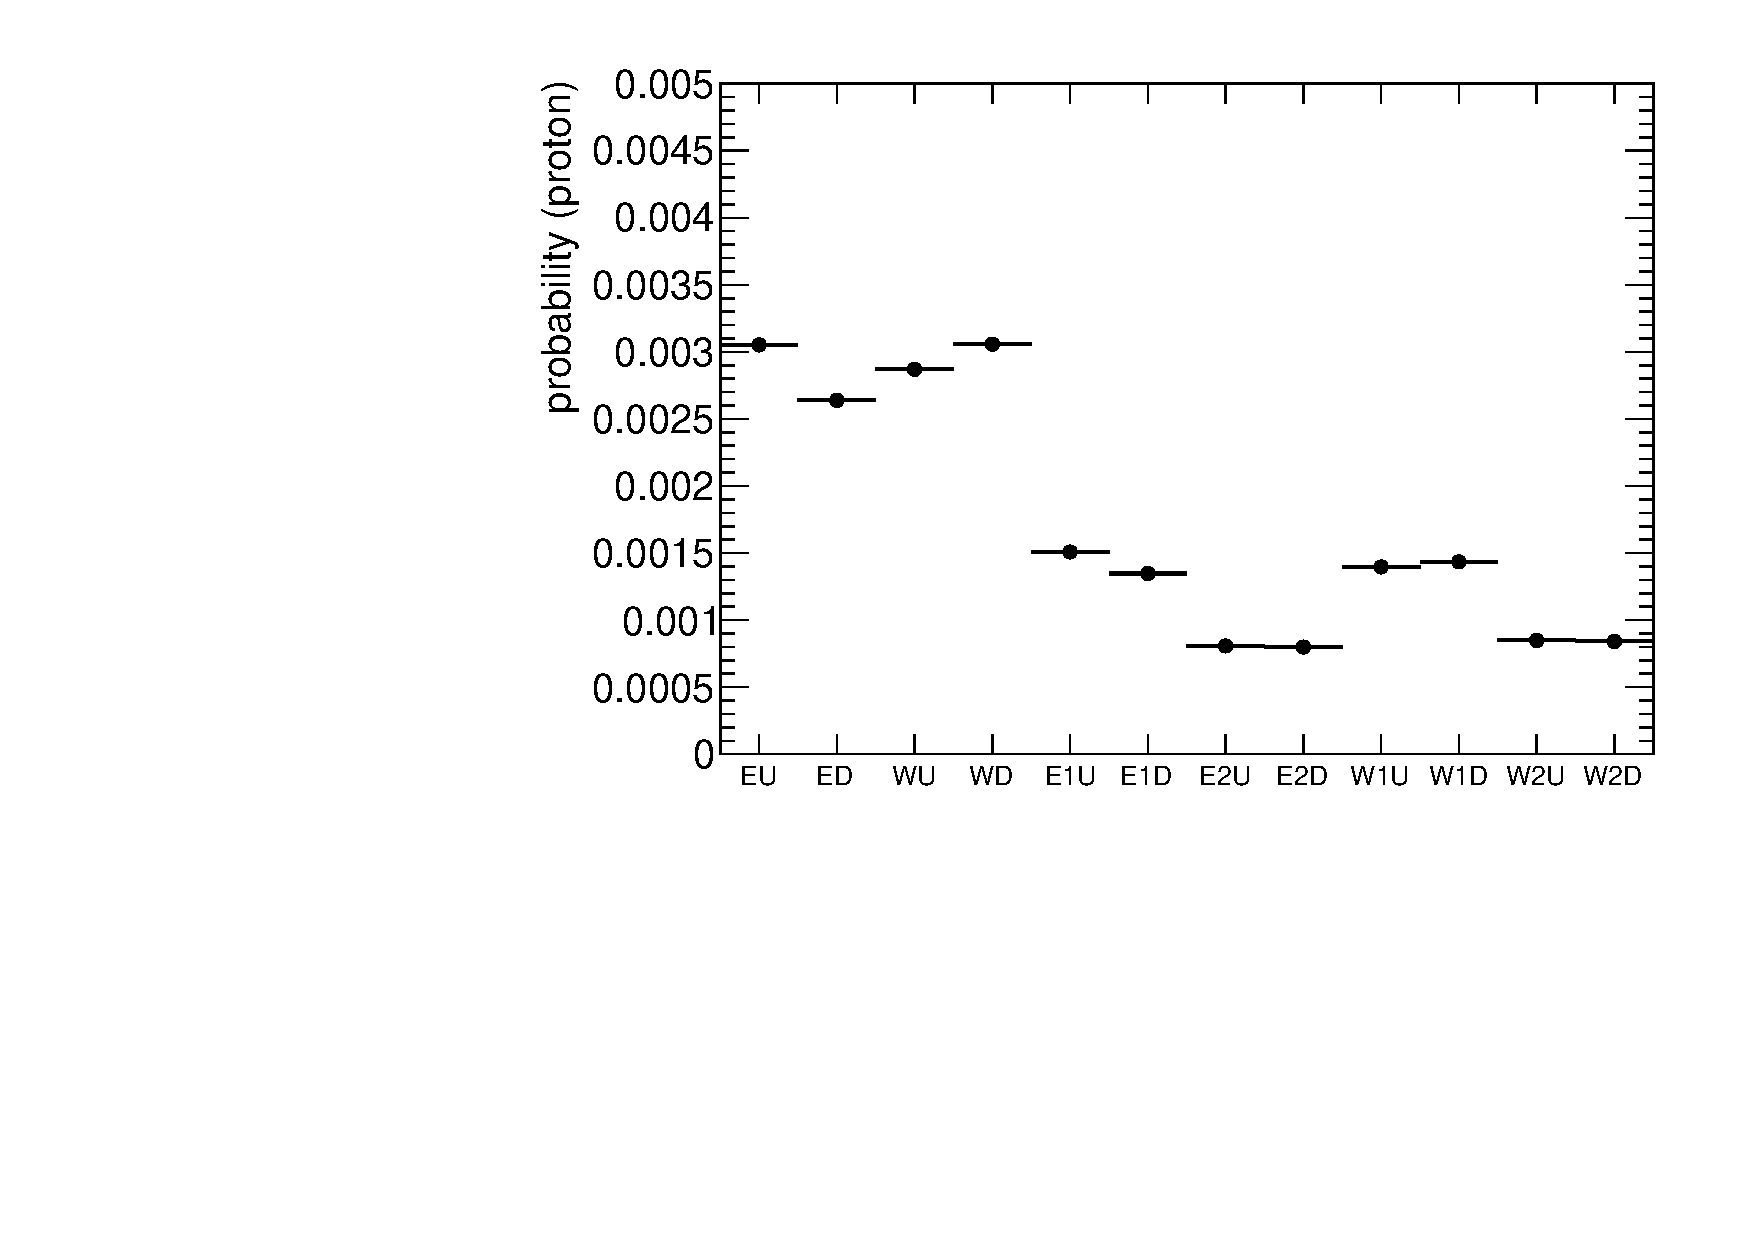
\includegraphics[width=\linewidth, page=1]{graphics/accidentals/accidentalBkg_1RP.pdf}}}
		\end{subfigure}
	}
	\quad
	\parbox{0.48\textwidth}{
		\centering
		\begin{subfigure}[b]{\linewidth}{
				\subcaptionbox{\label{fig:probCD}}{\includegraphics[width=\linewidth]{graphics/accidentals/accidentalBkg_2RP_cd.pdf}}}
		\end{subfigure}
	}%
	\caption[Proton overlay probability calculated from \textbf{Zerobias} trigger sample for SD and CD]{Proton overlay probability calculated from \textbf{Zerobias} trigger sample for SD (a) and CD (b, only proton global tracks used). The probability to observe accidental global tracks in RP in SD varies between $0.25-0.3\%$. Most of the accidental background in CD comes from the inelastic RP configuration.}
	
	 %\label{fig:probacc}
\end{figure}
\subsection{Accidental background in SD}
The background from accidentals in SD events was calculated from the \textbf{Zerobias} sample multiplied by the probability of observing the accidental proton track in the RP and corrected by the relevant trigger prescales $\frac{PS^{Zerobias}}{PS^{SDT}}$. Figure \ref{fig:hitSD} shows the proton hit position in E1U with the data-driven background contribution for the region of interest (a,b - proton global and local tracks; c,d - only proton global tracks). 
\begin{figure}[hb]
	\centering
	\parbox{0.48\textwidth}{
		\centering
		\begin{subfigure}[b]{\linewidth}{
				\subcaptionbox{\label{fig:E1UX}}{\includegraphics[width=\linewidth, page=14]{graphics/accidentals/accidentalBkg_1RP.pdf}}}
		\end{subfigure}
	}
	\quad
	\parbox{0.48\textwidth}{
		\centering
		\begin{subfigure}[b]{\linewidth}{
				\subcaptionbox{\label{fig:E1UY}}{\includegraphics[width=\linewidth, page=15]{graphics/accidentals/accidentalBkg_1RP.pdf}}}
		\end{subfigure}
	}
	\parbox{0.48\textwidth}{
		\centering
		\begin{subfigure}[b]{\linewidth}{
				\subcaptionbox{\label{fig:E1UglobalX}}{\includegraphics[width=\linewidth,page=14]{graphics/accidentals/accidentalBkg.pdf}}}
		\end{subfigure}
	}
	\quad
	\parbox{0.48\textwidth}{
		\centering
		\begin{subfigure}[b]{\linewidth}{
				\subcaptionbox{\label{fig:E1UglobalY}}{\includegraphics[width=\linewidth,page=15]{graphics/accidentals/accidentalBkg.pdf}}}
		\end{subfigure}
	}
	\caption[Proton hit position in SD using global+local proton tracks (a-b) and only global proton tracks]{Proton hit position in SD using global+local proton tracks (a-b) and only global proton tracks (c-d). The background contribution equals to about $10\%$.}
	 \label{fig:hitSD}
\end{figure}
Due to observe the same  accidental backround contribution  for global and global+local proton track $\left(\approx 10\%\right)$, also the $-t$ and $\xi$ distributions were checked (Figure \ref{fig:txiSD}). To reconstruct properly $-t$ and $\xi$ only global proton tracks were used. The flat background was observed in the $-t$ distribution. However, the $\xi$ distribution shows that most of the background is located around $\xi\approx 0$, which confirms the assumption that most of the accidental background comes from elastic, beam halo or low mass diffractive protons.
\begin{figure}[h]
	\centering
	\parbox{0.48\textwidth}{
		\centering
		\begin{subfigure}[b]{\linewidth}{
				\subcaptionbox{\label{fig:tSD}}{\includegraphics[width=\linewidth, page=33]{graphics/accidentals/accidentalBkg.pdf}}}
		\end{subfigure}
	}
	\quad
	\parbox{0.48\textwidth}{
		\centering
		\begin{subfigure}[b]{\linewidth}{
				\subcaptionbox{\label{fig:xiSD}}{\includegraphics[width=\linewidth, page=37]{graphics/accidentals/accidentalBkg.pdf}}}
		\end{subfigure}
	}
	\caption[$-t$ and $\xi$ distribution for WD arm in SD]{$-t$ and $\xi$ distribution for WD arm in SD. Accidental background suppressed for $0.02<\xi<0.4$.}
	 \label{fig:txiSD}
\end{figure}

 Additionally, the background begins to rise at $\xi\approx 0.4$. This probably comes from  true or fake tracks reconstructed in RP arising from showers happening outside the RP stations. Finally, the additional proton selection cuts were obtained for SD - the proton track is required to be a global track with $0.02 < \xi < 0.4$. The probability to observe the accidental proton in RP decreased to about $0.15\%$ (Figure \ref{fig:probSDcut}) and the accidental background contribution is about $5-10\%$ (Figure \ref{fig:tSDcut}).
 \begin{figure}[H]
 	\centering
 	\parbox{0.48\textwidth}{
 		\centering
 		\begin{subfigure}[b]{\linewidth}{
 				\subcaptionbox{\label{fig:probSDcut}}{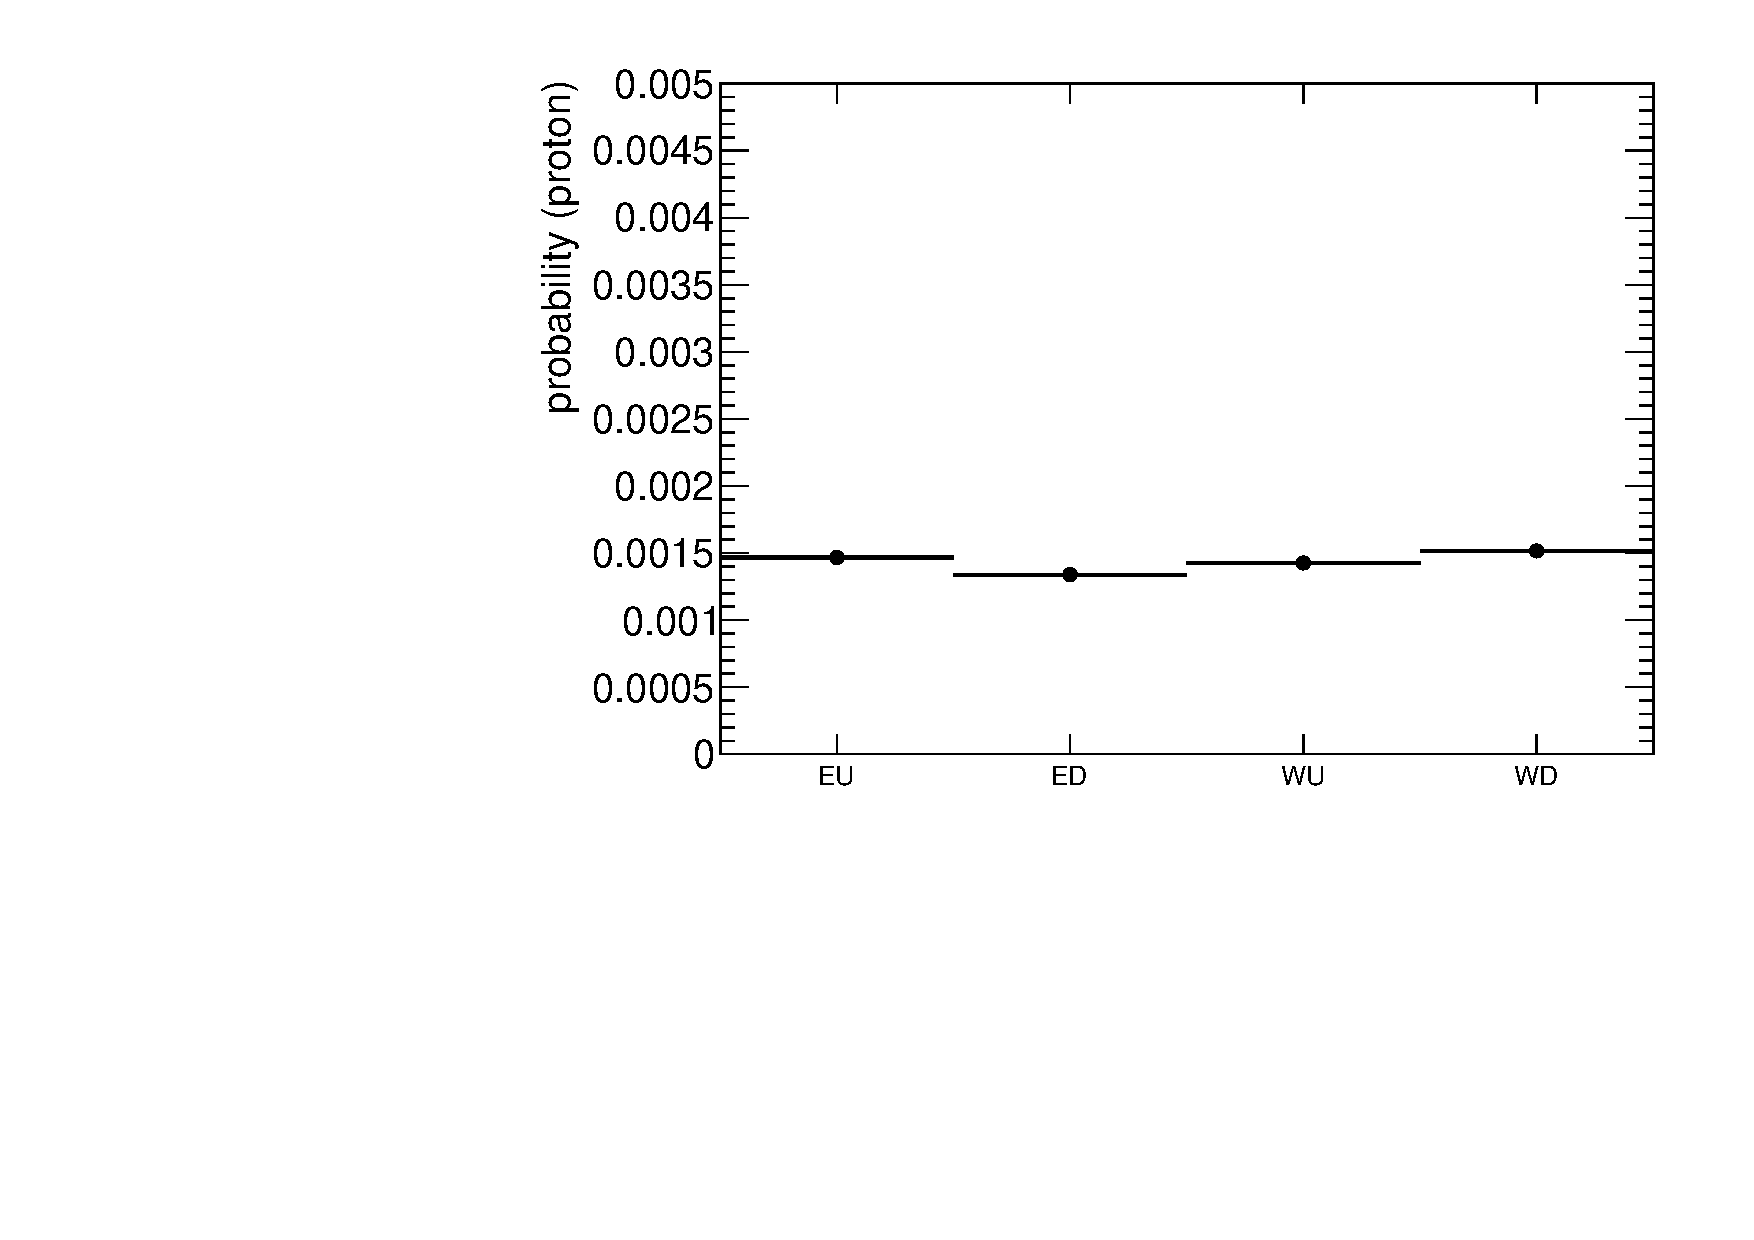
\includegraphics[width=\linewidth, page=1]{graphics/accidentals/accidentalBkg_XiCut2.pdf}}}
 		\end{subfigure}
 	}
 	\quad
 	\parbox{0.48\textwidth}{
 		\centering
 		\begin{subfigure}[b]{\linewidth}{
 				\subcaptionbox{\label{fig:tSDcut}}{\includegraphics[width=\linewidth, page=33]{graphics/accidentals/accidentalBkg_XiCut2.pdf}}}
 		\end{subfigure}
 	}
 	% \label{fig:xy_recoEff}
 	\caption[Proton overlay probability and $-t$ distribution for SD events with $0.02 < \xi < 0.4$]{Proton overlay probability (a) and $-t$ (b) distribution for SD events with $0.02 < \xi < 0.4$. The~probability to observe accidental proton in RP decreased to about $0.15\%$.}
 \end{figure}
 \begin{figure}[H]
 	\centering
 	\parbox{0.48\textwidth}{
 		\centering
 		\begin{subfigure}[b]{\linewidth}{
 				\subcaptionbox{\label{fig:xSDcut}}{\includegraphics[width=\linewidth, page=14]{graphics/accidentals/accidentalBkg_XiCut2.pdf}}}
 		\end{subfigure}
 	}
 	\quad
 	\parbox{0.48\textwidth}{
 		\centering
 		\begin{subfigure}[b]{\linewidth}{
 				\subcaptionbox{\label{fig:ySDcut}}{\includegraphics[width=\linewidth, page=15]{graphics/accidentals/accidentalBkg_XiCut2.pdf}}}
 		\end{subfigure}
 	}
 	\caption[Proton hit position in E1U for SD events with $0.02 < \xi < 0.4$.]{Proton hit position in E1U for SD events with $0.02 < \xi < 0.4$.}
 	% \label{fig:xy_recoEff}
 \end{figure}
 \begin{figure}[H]
 	\centering
 	\parbox{0.48\textwidth}{
 		\centering
 		\begin{subfigure}[b]{\linewidth}{
 				\subcaptionbox{\label{fig:ntrSDcut}}{\includegraphics[width=\linewidth, page=2]{graphics/accidentals/accidentalBkg_XiCut2.pdf}}}
 		\end{subfigure}
 	}
 	\quad
 	\parbox{0.48\textwidth}{
 		\centering
 		\begin{subfigure}[b]{\linewidth}{
 				\subcaptionbox{\label{fig:etaSDcut}}{\includegraphics[width=\linewidth, page=5]{graphics/accidentals/accidentalBkg_XiCut2.pdf}}}
 		\end{subfigure}
 	}
 	% \label{fig:xy_recoEff}
 	\caption[TPC-TOF related variables (TPC-TOF track multiplicity and $\eta$ of those tracks) for SD events with $0.02 < \xi < 0.4$.]{TPC-TOF related variables (TPC-TOF track multiplicity and $\eta$ of those tracks) for SD events with $0.02 < \xi < 0.4$. The background contribution is about $5-10\%$.}
 \end{figure}
 %\clearpage
 %\newpage
\subsection{Accidental background in CD}
The background from accidentals in CD events was calculated in the similar way to the SD. Only proton global tracks were used to calculate the probability of observing two accidental protons on the opposite sides of the IP. Figure \ref{fig:CDcoll} shows the collinearity distributions for inelastic (a) and elastic (b) RP configuration. 
\begin{figure}[H]
	\centering
	\parbox{0.48\textwidth}{
		\centering
		\begin{subfigure}[b]{\linewidth}{
				\subcaptionbox{\label{fig:accThetaX}}{\includegraphics[width=\linewidth, page=49]{graphics/accidentals/accidentalBkg_2RP_cd.pdf}}}
		\end{subfigure}
	}
	\quad
	\parbox{0.48\textwidth}{
		\centering
		\begin{subfigure}[b]{\linewidth}{
				\subcaptionbox{\label{fig:accThetaY}}{\includegraphics[width=\linewidth, page=55]{graphics/accidentals/accidentalBkg_2RP_cd.pdf}}}
		\end{subfigure}
	}
	\parbox{0.48\textwidth}{
		\centering
		\begin{subfigure}[b]{\linewidth}{
				\subcaptionbox{\label{fig:accTheta}}{\includegraphics[width=\linewidth, page=7]{graphics/accidentals/accidentalBkg_2RP_cd_scale.pdf}}}
		\end{subfigure}
	}
	% \label{fig:xy_recoEff}
	\caption[Collinearity distribution $\theta_X$ for inelastic and elastic RP configuration in CD]{Collinearity distribution $\theta_X$ for inelastic (a) and elastic (b) RP configuration in CD. The accidental background for elastic configuration is overestimated. The background was normalized to the signal in the first bin of the collinearity distribution (c).}
	\label{fig:CDcoll}
\end{figure}
The accidental background for the elastic configuration excess the $100\%$ and is overestimated. Two solutions were found to estimate the background in the elastic RP configuration:
\begin{enumerate}
	\item Require the protons to be anti-collinear $\left(\left(\delta\theta_x/\sigma_x\right)^2+\left(\delta\theta_y/\sigma_y\right)^2<3^2\right)$. 
\begin{figure}[H]
	\centering
	\parbox{0.48\textwidth}{
		\centering
		\begin{subfigure}[b]{\linewidth}{
				\subcaptionbox{\label{fig:accCDxiColl}}{\includegraphics[width=\linewidth, page=26]{graphics/accidentals/accidentalBkg_2RP_cd_Coll.pdf}}}
		\end{subfigure}
	}
	\quad
	\parbox{0.48\textwidth}{
		\centering
		\begin{subfigure}[b]{\linewidth}{
				\subcaptionbox{\label{fig:accCut}}{\includegraphics[width=\linewidth, page=1]{graphics/accidentals/accidentalBkg_2RP_cd_cut_NoColl.pdf}}}
		\end{subfigure}
	}
	\parbox{0.48\textwidth}{
		\centering
		\begin{subfigure}[b]{\linewidth}{
				\subcaptionbox{\label{fig:accThetaCut}}{\includegraphics[width=\linewidth, page=54]{graphics/accidentals/accidentalBkg_2RP_cd_cut_NoColl.pdf}}}
		\end{subfigure}
	}
	% \label{fig:xy_recoEff}
	\caption[x]{$\xi$ distribution of protons in EU arm with collinearity cut. The background is suppressed for  $0.02<\xi_1,\xi_2<0.4$ and the proton overlay probability is reduced to $2\cdot10^{-5}$. The accidental background contribution was reduced to about $5\%$ with this cut.}
\end{figure}
	The $\xi$ distribution  with collinearity cut, as shown in Figure \ref{fig:accCDxiColl}, was checked and it was found that the proton tracks should be required to be global tracks with $0.02<\xi_1,\xi_2<0.4$. With this cuts the probability of observing two accidental protons was reduced to about $2\cdot10^{-5}$ for all RP configurations (Figure \ref{fig:accCut}). Additionally, the overestimation of the background was not observed in the collinearity distribution (Figure \ref{fig:accThetaCut}) and the accidental background contribution decreased to about $5\%$.
\begin{figure}[H]
	\centering
	\parbox{0.48\textwidth}{
		\centering
		\begin{subfigure}[b]{\linewidth}{
				\subcaptionbox{\label{fig:accCDxielCut}}{\includegraphics[width=\linewidth, page=35]{graphics/accidentals/accidentalBkg_2RP_cd_cut_NoColl.pdf}}}
		\end{subfigure}
	}
	\quad
	\parbox{0.48\textwidth}{
		\centering
		\begin{subfigure}[b]{\linewidth}{
				\subcaptionbox{\label{fig:accCDtelCut}}{\includegraphics[width=\linewidth, page=43]{graphics/accidentals/accidentalBkg_2RP_cd_cut_NoColl.pdf}}}
		\end{subfigure}
	}
	\parbox{0.48\textwidth}{
		\centering
		\begin{subfigure}[b]{\linewidth}{
				\subcaptionbox{\label{fig:accCDxiinelCut}}{\includegraphics[width=\linewidth, page=33]{graphics/accidentals/accidentalBkg_2RP_cd_cut_NoColl.pdf}}}
		\end{subfigure}
	}
	\quad
	\parbox{0.48\textwidth}{
		\centering
		\begin{subfigure}[b]{\linewidth}{
				\subcaptionbox{\label{fig:accCDtinelCut}}{\includegraphics[width=\linewidth, page=41]{graphics/accidentals/accidentalBkg_2RP_cd_cut_NoColl.pdf}}}
		\end{subfigure}
	}
	% \label{fig:xy_recoEff}
	\caption[x]{$\xi$ and $-t$ in elastic and inelastic RP configuration measured with EU. The background is reduced to about $5\%$ in both RP configurations.}
\end{figure}
	\item Normalize the background to the signal in the first bin  of the collinearity distribution (Figure \ref{fig:accTheta}). Here it was assumed that all collinear protons are background protons and the upper limit for the background was set. Also the scale factor for the background was found. Similar to the first method, it was found that the background is supressed for $0.02<\xi_1,\xi_2<0.4$ and varies between $2-3\%$ (Figure \ref{fig:xecCutAcc} b-d). The collinearity cut is not required anymore.
\begin{figure}[H]
	\centering
	\parbox{0.48\textwidth}{
		\centering
		\begin{subfigure}[b]{\linewidth}{
				\subcaptionbox{\label{fig:accCDxiel2}}{\includegraphics[width=\linewidth, page=30]{graphics/accidentals/accidentalBkg_2RP_cd_scale.pdf}}}
		\end{subfigure}
	}
	\quad
	\parbox{0.48\textwidth}{
		\centering
		\begin{subfigure}[b]{\linewidth}{
				\subcaptionbox{\label{fig:accCDxiCut2}}{\includegraphics[width=\linewidth, page=30]{graphics/accidentals/accidentalBkg_2RP_cd_Cut_scale.pdf}}}
		\end{subfigure}
	}
	\parbox{0.48\textwidth}{
		\centering
		\begin{subfigure}[b]{\linewidth}{
				\subcaptionbox{\label{fig:accCDtelCut2}}{\includegraphics[width=\linewidth, page=38]{graphics/accidentals/accidentalBkg_2RP_cd_Cut_scale.pdf}}}
		\end{subfigure}
	}
	\quad
	\parbox{0.48\textwidth}{
		\centering
		\begin{subfigure}[b]{\linewidth}{
				\subcaptionbox{\label{fig:accCDCollCut2}}{\includegraphics[width=\linewidth, page=4]{graphics/accidentals/accidentalBkg_2RP_cd_Cut_scale.pdf}}}
		\end{subfigure}
	}
	% \label{fig:xy_recoEff}
	\caption[x]{$\xi$ distribution in CD with the accidental background normalized to the signal in the first bin of the collinearity distribution (Figure \ref{fig:accTheta}). Most of the accidental background located outside the $0.02<\xi_1,\xi_2<0.4$ region. The background reduced to about $2-3\%$ in $\xi$, $-t$ and collinearity distributions with $0.02<\xi_1,\xi_2<0.4$ cut applied.}
	\label{fig:xecCutAcc}
\end{figure}
\end{enumerate}
\begin{figure}[H]
	\centering
	\parbox{0.48\textwidth}{
		\centering
		\begin{subfigure}[b]{\linewidth}{
				\subcaptionbox{\label{fig:accCDxin}}{\includegraphics[width=\linewidth, page=61]{graphics/accidentals/accidentalBkg_2RP_cd_cut_NoColl.pdf}}}
		\end{subfigure}
	}
	\quad
	\parbox{0.48\textwidth}{
		\centering
		\begin{subfigure}[b]{\linewidth}{
				\subcaptionbox{\label{fig:accCDyin}}{\includegraphics[width=\linewidth, page=62]{graphics/accidentals/accidentalBkg_2RP_cd_cut_NoColl.pdf}}}
		\end{subfigure}
	}
	\parbox{0.48\textwidth}{
		\centering
		\begin{subfigure}[b]{\linewidth}{
				\subcaptionbox{\label{fig:accCDxel}}{\includegraphics[width=\linewidth, page=69]{graphics/accidentals/accidentalBkg_2RP_cd_cut_NoColl.pdf}}}
		\end{subfigure}
	}
	\quad
	\parbox{0.48\textwidth}{
		\centering
		\begin{subfigure}[b]{\linewidth}{
				\subcaptionbox{\label{fig:accCDyel}}{\includegraphics[width=\linewidth, page=70]{graphics/accidentals/accidentalBkg_2RP_cd_cut_NoColl.pdf}}}
		\end{subfigure}
	}
	% \label{fig:xy_recoEff}
	\caption[x]{Proton hit positions for E2U in inelastic (a, b) and elastic (c,d) RP configuration with $0.02<\xi_1,\xi_2<0.4$ cut applied. The background reduced to about $2-4\%$ in both RP configurations.}
\end{figure}
\begin{figure}[H]
	\centering
	\parbox{0.48\textwidth}{
		\centering
		\begin{subfigure}[b]{\linewidth}{
				\subcaptionbox{\label{fig:accCDntrinel}}{\includegraphics[width=\linewidth, page=12]{graphics/accidentals/accidentalBkg_2RP_cd_Cut_scale.pdf}}}
		\end{subfigure}
	}
	\quad
	\parbox{0.48\textwidth}{
		\centering
		\begin{subfigure}[b]{\linewidth}{
				\subcaptionbox{\label{fig:accCDetael}}{\includegraphics[width=\linewidth, page=24]{graphics/accidentals/accidentalBkg_2RP_cd_Cut_scale.pdf}}}
		\end{subfigure}
	}
	\parbox{0.48\textwidth}{
		\centering
		\begin{subfigure}[b]{\linewidth}{
				\subcaptionbox{\label{fig:accCDntrel}}{\includegraphics[width=\linewidth, page=13]{graphics/accidentals/accidentalBkg_2RP_cd_Cut_scale.pdf}}}
		\end{subfigure}
	}
	\quad
	\parbox{0.48\textwidth}{
		\centering
		\begin{subfigure}[b]{\linewidth}{
				\subcaptionbox{\label{fig:accCDetainel}}{\includegraphics[width=\linewidth, page=25]{graphics/accidentals/accidentalBkg_2RP_cd_Cut_scale.pdf}}}
		\end{subfigure}
	}
	% \label{fig:xy_recoEff}
	\caption[x]{TPC-TOF related variables (TPC-TOF track multiplicity and $\eta$ of those tracks) for CD events with $0.02<\xi_1,\xi_2<0.4$. The background contribution is about $0.5\%$.}
\end{figure}

\subsection{TPC related distributions with additional proton selection cuts}
The additional proton selection $\xi\left(\xi_1,\xi_2\right)$ cuts reduce the statistics of about $20\%$ and $50\%$ for SD and CD, respectively. The most significant background reduction was observed mainly in CD. Figure \ref{fig:reduction} shows the comparison of the $p_T$ (c, f) and $\eta$ (b, e) distibutions with and without the $\xi\left(\xi_1,\xi_2\right)$ cuts applied. In spite of the reduction of the background, the shape of those distributions did not change. Although, the TPC-TOF track multiplicity distribution changed with above cuts applied (Figure \ref{fig:reduction} a, d). The rest of the accidental background has to be  subtracted statistically.
\begin{figure}[H]
	\centering
	\parbox{0.31\textwidth}{
		\centering
		\begin{subfigure}[b]{\linewidth}{
				\subcaptionbox{\label{fig:redSDntr}}{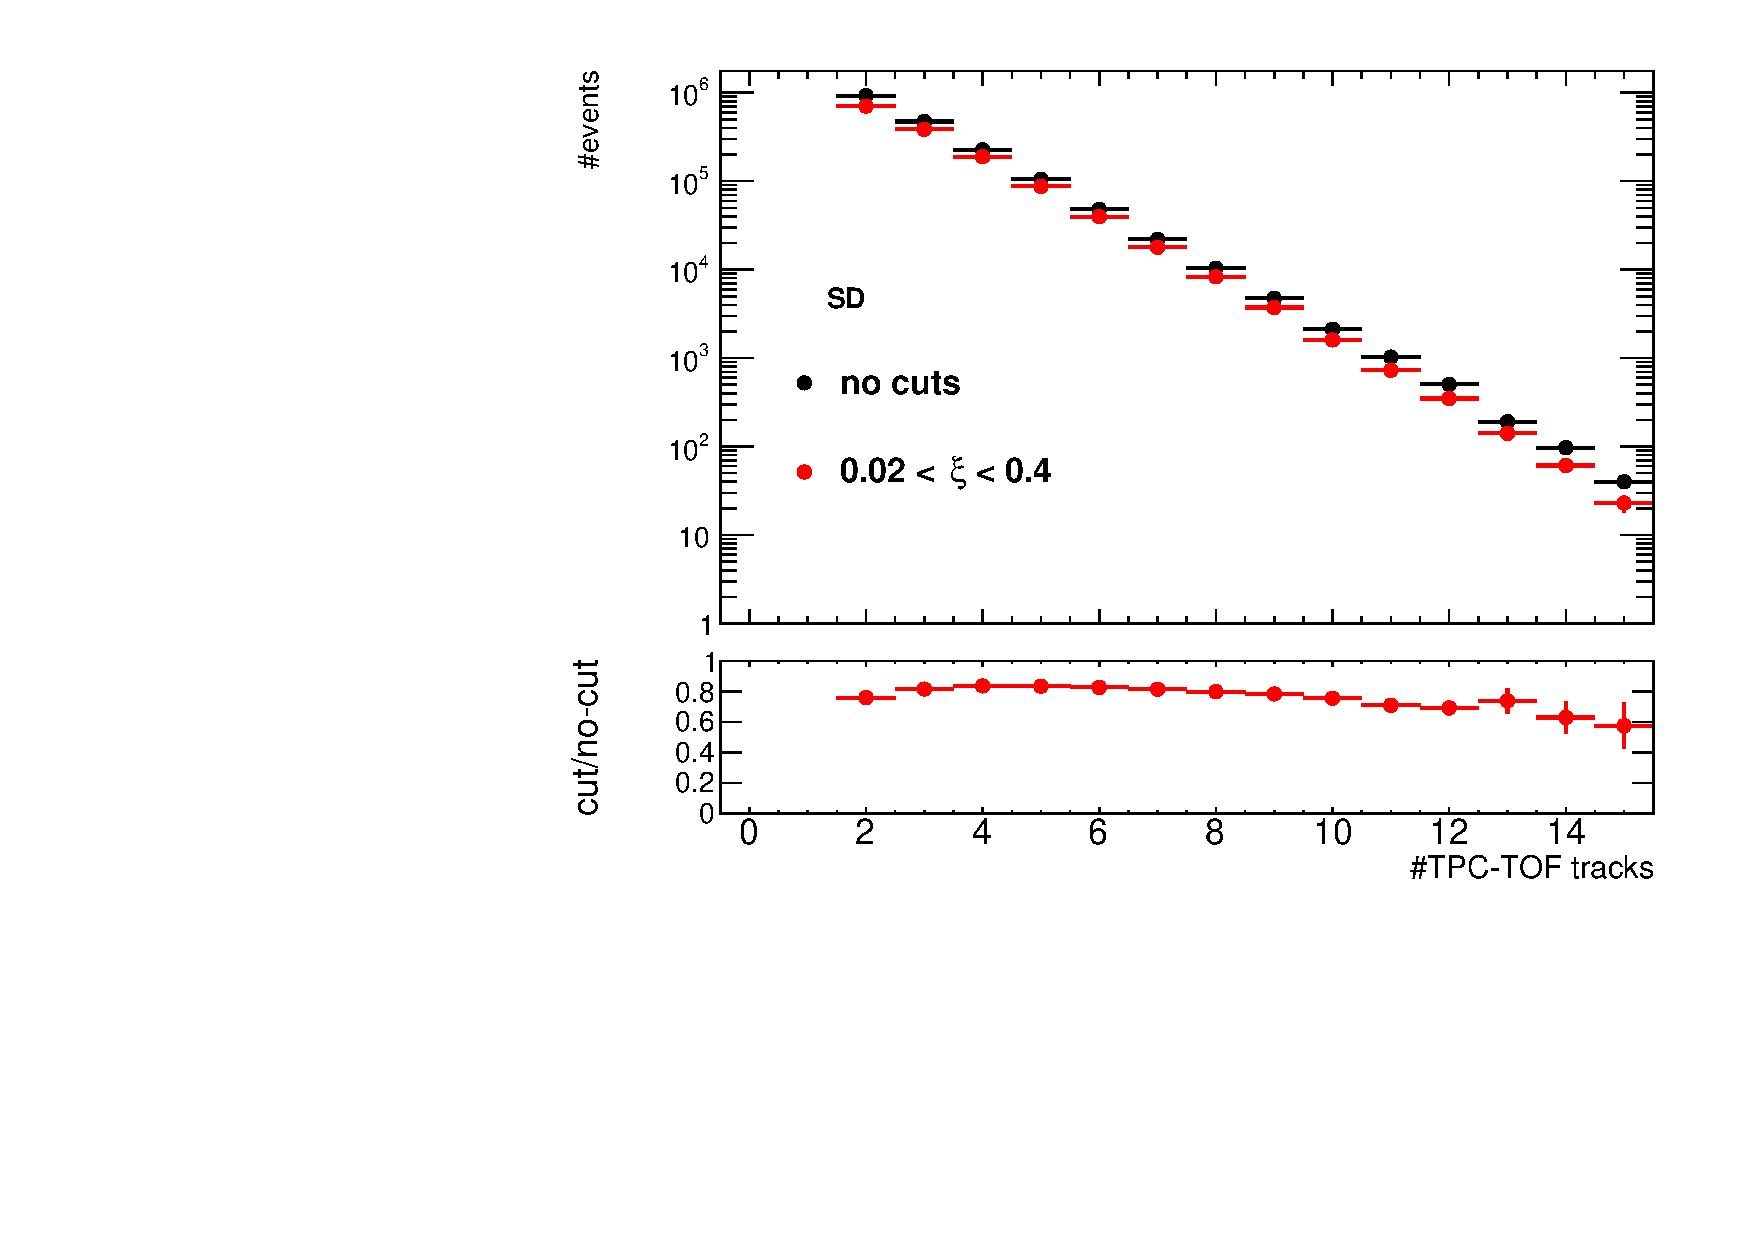
\includegraphics[width=\linewidth, page=1]{graphics/accidentals/compareCuts.pdf}}}
		\end{subfigure}
	}
	\quad
	\parbox{0.31\textwidth}{
		\centering
		\begin{subfigure}[b]{\linewidth}{
				\subcaptionbox{\label{fig:redSDeta}}{\includegraphics[width=\linewidth, page=3]{graphics/accidentals/compareCuts.pdf}}}
		\end{subfigure}
	}
	\quad
	\parbox{0.31\textwidth}{
		\centering
		\begin{subfigure}[b]{\linewidth}{
				\subcaptionbox{\label{fig:redSDpt}}{\includegraphics[width=\linewidth, page=5]{graphics/accidentals/compareCuts.pdf}}}
		\end{subfigure}
	}
	\parbox{0.31\textwidth}{
		\centering
		\begin{subfigure}[b]{\linewidth}{
				\subcaptionbox{\label{fig:redCDntr}}{\includegraphics[width=\linewidth, page=2]{graphics/accidentals/compareCuts.pdf}}}
		\end{subfigure}
	}
	\quad
	\parbox{0.31\textwidth}{
		\centering
		\begin{subfigure}[b]{\linewidth}{
				\subcaptionbox{\label{fig:redCDeta}}{\includegraphics[width=\linewidth, page=4]{graphics/accidentals/compareCuts.pdf}}}
		\end{subfigure}
	}
	\quad
	\parbox{0.31\textwidth}{
		\centering
		\begin{subfigure}[b]{\linewidth}{
				\subcaptionbox{\label{fig:redCDpt}}{\includegraphics[width=\linewidth, page=6]{graphics/accidentals/compareCuts.pdf}}}
		\end{subfigure}
	}
   
	\caption[TPC-TOF related distributions with and without additional proton track selection cuts applied in SD and CD]{TPC-TOF related distributions with and without additional proton track selection cuts applied in SD (a-c) and CD (d-f). The additional proton selection $\xi\left(\xi_1,\xi_2\right)$ cuts reduce the statistics of about $20\%$ and $50\%$ for SD and CD, respectively.}
	\label{fig:reduction}
\end{figure}
\section{Particle Identification}

